TODO: apraksti grafikiem un tabula līdz ko būs final version.


\begin{figure}[h] 
   \centering
   \subcaptionbox{mBERT latviešu treniņdatu kopa}{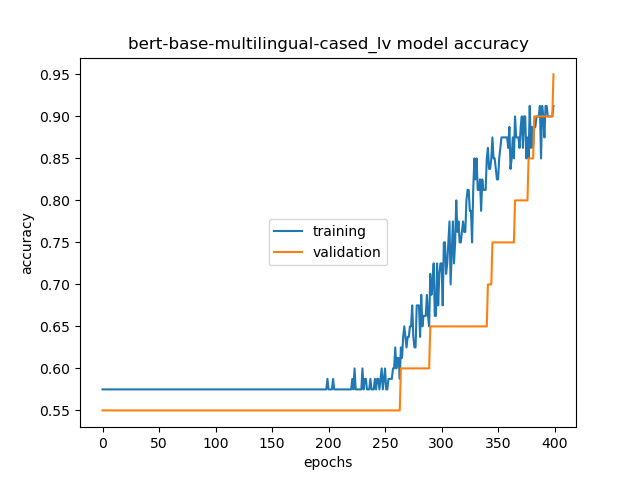
\includegraphics[width=0.49\linewidth,trim={0 0.1cm 0 0},clip]{graphs/bert-base-multilingual-cased_lv-accuracy.png}}
   \subcaptionbox{mBERT mašīntulkoto latviešu treniņdatu kopa}{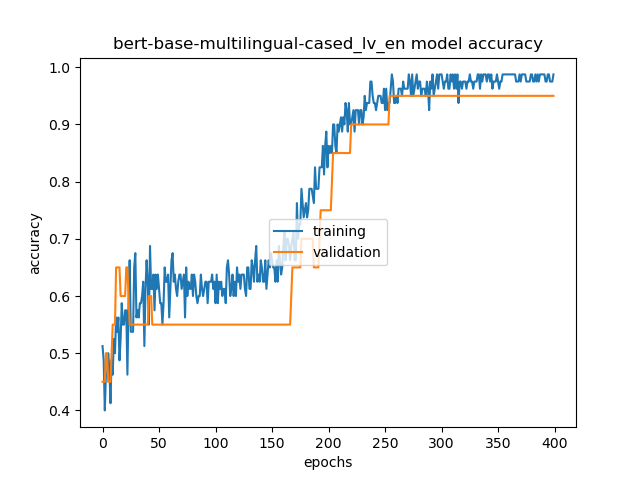
\includegraphics[width=0.49\linewidth,trim={0 0.1cm 0 0},clip]{graphs/bert-base-multilingual-cased_lv_en-accuracy.png}}
   \caption{caption} 
   \label{fig:bert}
\end{figure}


\begin{figure}[h] 
   \centering
   \subcaptionbox{mBERT apvienotā treniņdatu kopa}{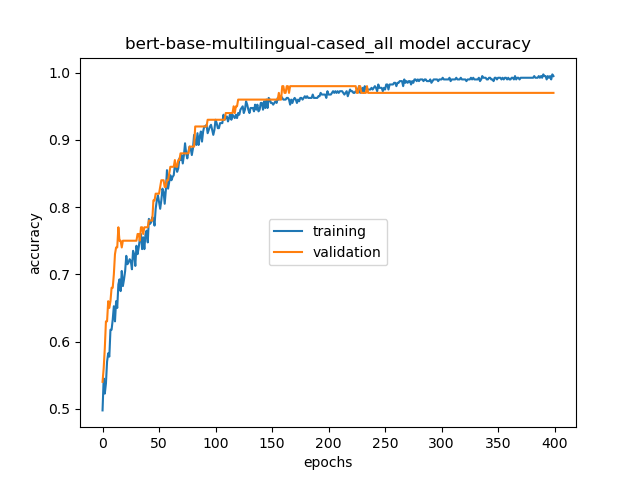
\includegraphics[width=0.49\linewidth,trim={0 0.1cm 0 0},clip]{graphs/bert-base-multilingual-cased_all-accuracy.png}}
   \subcaptionbox{mBERT apvienotā mašīntulkoto treniņdatu kopa}{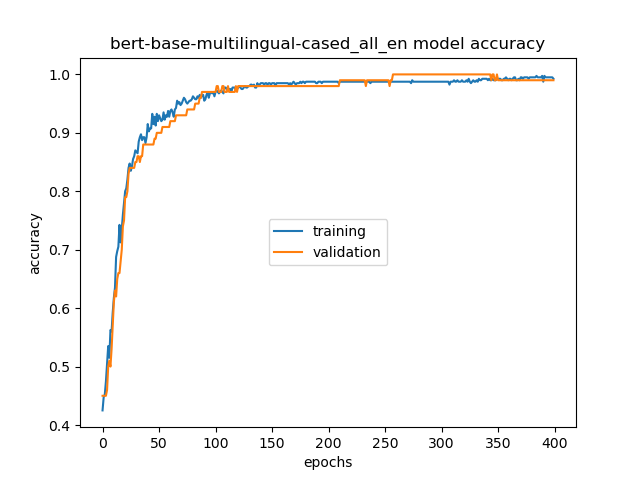
\includegraphics[width=0.49\linewidth,trim={0 0.1cm 0 0},clip]{graphs/bert-base-multilingual-cased_all_en-accuracy.png}}
   \caption{caption} 
   \label{fig:bert-all}
\end{figure}


\begin{figure}[h] 
   \centering
   \subcaptionbox{mBERT angļu treniņdatu kopa}{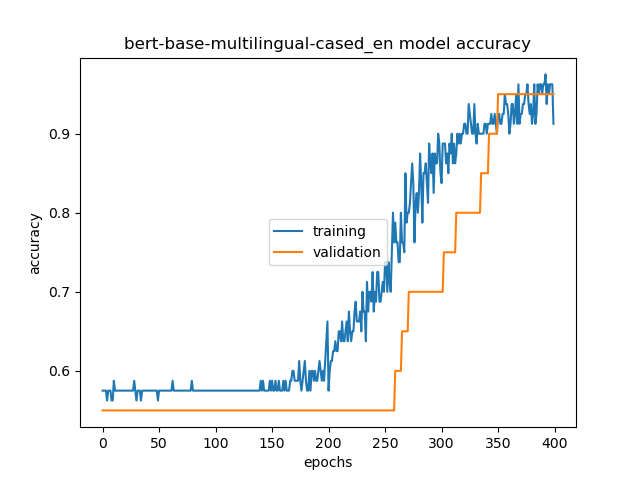
\includegraphics[width=0.49\linewidth,trim={0 0.1cm 0 0},clip]{graphs/bert-base-multilingual-cased_en-accuracy.png}}
   \subcaptionbox{XLM-RoBERTa angļu treniņdatu kopa}{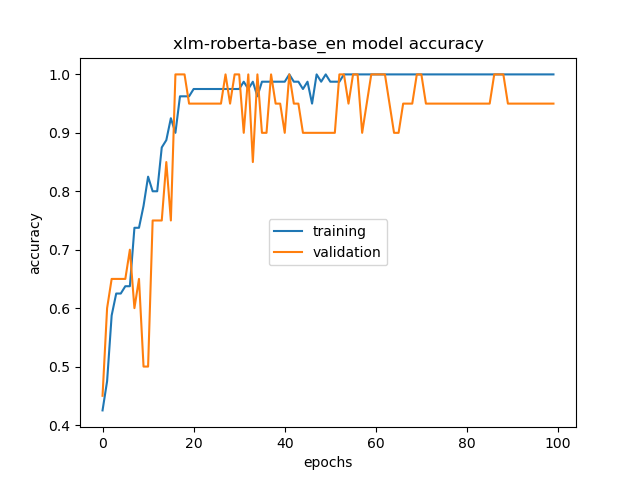
\includegraphics[width=0.49\linewidth,trim={0 0.1cm 0 0},clip]{graphs/xlm-roberta-base_en-accuracy.png}}
   \caption{caption} 
   \label{fig:bert-xlm-en}
\end{figure}
